% !TEX encoding = UTF-8
% !TEX TS-program = pdflatex
% !TEX root = ../tesi.tex

%**************************************************************
\chapter{Verifica e validazione}
\label{cap:verifica-validazione}
%**************************************************************

\intro{In questo capitolo viene descritto come sono state affrontate le attività di verifica e
validazione del prodotto.}\\

%**************************************************************
\section{Considerazioni}
\label{sec:considerazioni}

Nel piano di lavoro, redatto dal tutor aziendale e approvato dal tutor interno, veniva menzionato lo sviluppo del test automatici come un obiettivo opzionale, preferendo ad essi nuove feature. Per questo, in accordo con il mio tutor aziendale, mi sono dedicato maggiormente all’implementazione e documentazione di esse. Ho comunque avuto modo di effettuare dei test manuali sull’applicativo, verificando il suo corretto funzionamento. I test automatici, che per mancanza di tempo non sono stati sviluppati, verranno implementati successivamente dall’azienda, per provare l’effettiva qualità del software prodotto.

\section{Analisi statica}

Per effettuare l’analisi statica del codice, non sono stati utilizzati particolati strumenti come per esempio linter, questo perché ho ritenuto che l’IDE PyCharm fornisse aiuti più che sufficienti. È noto che PyCharm suggerisce correzioni per eventuali errori introdotti nel codice e miglioramenti durante la scrittura del codice.
In particolare, PyCharm segnala, più comunemente:
\begin{itemize}
	\item incoerenza tra tipi di dati coinvolti in un’istruzione se utilizzati i type hint;
	\item codice non raggiungibile dal flusso di controllo;
	\item variabili dichiarate ma non utilizzate;
	\item metodi dichiarati ma non implementati;
	\item errori di sintassi;
	\item controllo delle librerie importate ma non utilizzate.
\end{itemize}

Inoltre, per concludere, PyCharm offre due funzionalità che ho utilizzato spesso, una è la formattazione automatica del codice e l’altra l’importazione e organizzazione delle classi, sempre automatica.

\section{Analisi dinamica}

Per quanto concerne l’analisi dinamica, nel corso dell’intera fase di codifica, ho potuto verificare il codice utilizzando lo strumento integrato di PyCharm per effettuare il debug, insieme alla libreria Python logger. I test sono stati tutti effettuati manualmente, a questo fine sono state create tre macchine virtuali connesse nella stessa rete. La prima centralizza i servizi utilizzati quali redis e rabbitmq ed inoltre il modulo denominato master, le altre due macchine invece effettuavano lo scraping utilizzando il modulo worker collegandosi ai servizi offerti dalla prima macchina. \newline{}
Al termine di una run di test viene effettuato un lavoro di analisi dei log. Utilizzando una libreria python da me sviluppata, si può avere una visualizzazione grafica delle informazioni ritenute interessanti dall'analista, facilitando il lavoro. Un esempio concreto è l'analisi dell'utilizzo di memoria da parte del modulo durante le varie iterazioni, una rappresentazione grafica può risultare più facilmente intepretabile.

\begin{figure}[!h] 
    \centering 
    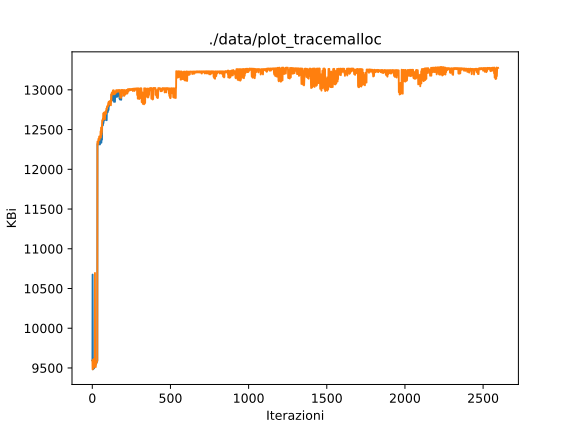
\includegraphics[width=0.6\columnwidth]{chapter5-verify/tracemalloc.png} 
    \caption{Visualizzazione utilizzo memoria}
    \label{fig:visualizzazione-utilizzo-memoria} 
\end{figure}




